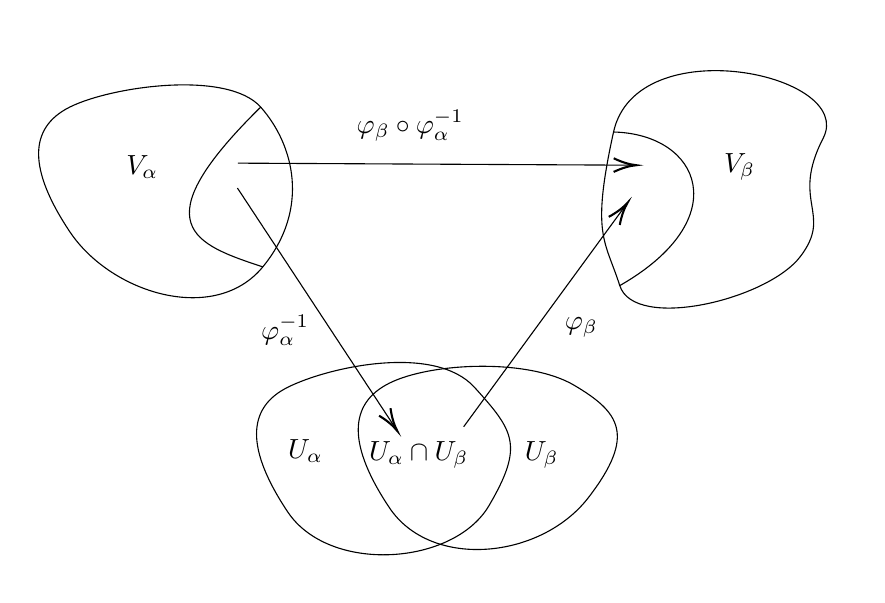
\begin{tikzpicture}[x=0.75pt,y=0.75pt,yscale=-1,xscale=1]
    %uncomment if require: \path (0,301); %set diagram left start at 0, and has height of 301

    %Shape: Polygon Curved [id:ds7545552056106698] 
    \draw   (50,45) .. controls (70,35) and (126,27) .. (142,45) .. controls (158,63) and (166,94) .. (143,122) .. controls (120,150) and (70,135) .. (50,105) .. controls (30,75) and (30,55) .. (50,45) -- cycle ;
    %Shape: Polygon Curved [id:ds5522702672450327] 
    \draw   (312,57) .. controls (323,7) and (429,29) .. (413,60) .. controls (397,91) and (418,96) .. (402,117) .. controls (386,138) and (322,153) .. (315,131) .. controls (308,109) and (301,107) .. (312,57) -- cycle ;
    %Curve Lines [id:da21169301483212177] 
    \draw    (142,45) .. controls (84,102) and (110,111) .. (143,122) ;
    %Curve Lines [id:da030881504774420643] 
    \draw    (312,57) .. controls (354,58) and (371,99) .. (315,131) ;
    %Shape: Polygon Curved [id:ds7639047336485658] 
    \draw   (155,180) .. controls (175,170) and (226,159) .. (245,180) .. controls (264,201) and (269,208) .. (252,237) .. controls (235,266) and (175,270) .. (155,240) .. controls (135,210) and (135,190) .. (155,180) -- cycle ;
    %Shape: Polygon Curved [id:ds6261763207033869] 
    \draw   (204,178) .. controls (224,168) and (271,166) .. (293,179) .. controls (315,192) and (323,203) .. (300,233) .. controls (277,263) and (224,268) .. (204,238) .. controls (184,208) and (184,188) .. (204,178) -- cycle ;
    %Straight Lines [id:da16391710195567155] 
    \draw    (239.8,199) -- (317.62,92.61) ;
    \draw [shift={(318.8,91)}, rotate = 126.18] [color={rgb, 255:red, 0; green, 0; blue, 0 }  ][line width=0.75]    (10.93,-3.29) .. controls (6.95,-1.4) and (3.31,-0.3) .. (0,0) .. controls (3.31,0.3) and (6.95,1.4) .. (10.93,3.29)   ;
    %Straight Lines [id:da31384654750788643] 
    \draw    (130.8,84) -- (206.7,199.33) ;
    \draw [shift={(207.8,201)}, rotate = 236.65] [color={rgb, 255:red, 0; green, 0; blue, 0 }  ][line width=0.75]    (10.93,-3.29) .. controls (6.95,-1.4) and (3.31,-0.3) .. (0,0) .. controls (3.31,0.3) and (6.95,1.4) .. (10.93,3.29)   ;
    %Straight Lines [id:da13626397217094843] 
    \draw    (131,72) -- (321,72.99) ;
    \draw [shift={(323,73)}, rotate = 180.3] [color={rgb, 255:red, 0; green, 0; blue, 0 }  ][line width=0.75]    (10.93,-3.29) .. controls (6.95,-1.4) and (3.31,-0.3) .. (0,0) .. controls (3.31,0.3) and (6.95,1.4) .. (10.93,3.29)   ;

    % Text Node
    \draw (76,67) node [anchor=north west][inner sep=0.75pt]   [align=left] {$\displaystyle V_{\alpha }$};
    % Text Node
    \draw (364,66) node [anchor=north west][inner sep=0.75pt]   [align=left] {$\displaystyle V_{\beta }$};
    % Text Node
    \draw (154,204) node [anchor=north west][inner sep=0.75pt]   [align=left] {$\displaystyle U_{\alpha }$};
    % Text Node
    \draw (268,205) node [anchor=north west][inner sep=0.75pt]   [align=left] {$\displaystyle U_{\beta }$};
    % Text Node
    \draw (193,205) node [anchor=north west][inner sep=0.75pt]   [align=left] {$\displaystyle U_{\alpha } \cap U_{\beta }$};
    % Text Node
    \draw (141,144) node [anchor=north west][inner sep=0.75pt]   [align=left] {$\displaystyle \varphi _{\alpha }^{-1}$};
    % Text Node
    \draw (287.3,145) node [anchor=north west][inner sep=0.75pt]   [align=left] {$\displaystyle \varphi _{\beta }$};
    % Text Node
    \draw (187,45) node [anchor=north west][inner sep=0.75pt]   [align=left] {$\displaystyle \varphi _{\beta } \circ \varphi _{\alpha }^{-1}$};
\end{tikzpicture}